%!TEX root = ../docu.tex
\section{Grundlagen}

\subsection{Mobile Anwendungen}

Software und Services können auf verschiedenen Wegen für mobile Endgeräte entwickelt und angeboten werden. Aktuelle Plattformen wie Android\footnote{http://developer.android.com/index.html} von Google oder iOS\footnote{https://developer.apple.com/devcenter/ios/index.action} von Apple ermöglichen das Ausführen von Software durch den Benutzer.

Hierbei haben sich zwei Arten von Applikationen durchgesetzt. Beide bieten gewisse Vor- und Nachteile die im folgenden Abschnitt näher betrachtet werden.

\subsubsection{Webapplikationen}

Webapplikationen sind Applikationen die über einen Webbrowser auf dem Gerät abgerufen werden. Diese Applikationen werden von Betreibern von Websiten zur Verfügung gestellt und laufen unabhängig von der normalen Webpräsenz.

Durch verschiedene Kennungen kann der Webserver erkennen, ob Besucher der Webseiten von einem mobilen Endgerät aus auf die zur Verfügung gestellten Inhalte zugreifen wollen und anbietet daraufhin eine Webapplikation an.

Diese Form der Anwendungen ist in Unternehmen sehr beliebt. So können verschiedene IT-Systeme und Geschäftsprozesse ortsunabhängig von mobilen Geräten aus gesteuert und angezeigt werden.

Diese Art der Applikationen hat einen großen Vorteil für die Administration von mobilen Endgeräten im Unternehmen. So ist es möglich die Installation von nativen Applikationen gänzlich zu verbieten um sensible Daten auf den Gerät vor Dritten zu schützen. Was native Applikationen sind wird im Kapitel \ref{natand} erläutert. Dennoch können Anwendungen über den Webbrowser des Gerätes aufgerufen und verwendet werden.

VPN\footnote{engl. Virtuell Private LAN}-Lösungen unterstützen diese Verfahrensweise in dem sie den Benutzer im unternehmensinternen Internet\footnote{Intranet} festhalten und nur das Öffnen der Webapplikation im Unternehmensnetzwerk erlauben.

Der Sinn solcher Applikation ist neben der Plattformunabhängigkeit eine Ersparnis an Zeit und Kosten für bestimmte Unternehmensprozesse.

Ein Beispiel sind Geräte für Kassensysteme in Bars und Restaurants oder Geräte im Einsatz in Lagerhallen. Im Außendienst lösen Tablets und Smartphones immer mehr das Notebooks als Hauptwerkzeug der im Außendienst tätigen Mitarbeiter ab. Verschiedene Analysten von Marktforschungsgruppen melden vermehrt, dass Tablet-PCs und Smartphones das Notebook auf lange Sicht ablösen werden\cite{blogpost_1}.

Viele Unternehmen weltweit\cite{news_1} profitieren von dem Trend von \textit{BYOD}\footnote{engl. bring your own device}, welcher übersetzt soviel bedeutet wie, dass Mitarbeiter private Technik für die Arbeit nutzen dürfen. Vertreiber und Hersteller von IT-Komponenten \emph{Hewlett Packard} bietet verschiedene Hardware zur Unterstützung und Umsetzung an\footnote{http://h17007.www1.hp.com/de/de/solutions/technology/BYOD/}.

 Um \textit{BOYD} zu nutzen, können sich Mitarbeiter in das Unternehmensnetzwerk verbinden und Webapplikationen nutzen. Diese Maßnahmen sind oft mit Schulungen und Einweisungen verbunden und sollen die Produktivität erhöhen ohne hohe Kosten für Geräte und Mobilfunkverträge zu erzeugen.

\subsubsection{Native Applikationen}
\label{natand}

Native Applikationen können in einer Art Onlineshop der jeweiligen Zielplattform erworben oder kostenlos heruntergeladen werden. Je nach Plattform variiert hier die Verfahrensweise und Möglichkeit der Bezahlung.

Einmal erworbene Applikationen sind dabei immer für den Nutzer verfügbar. Diese Onlineshops bieten auch die Möglichkeit vorhandene Software auf die aktuellste Version zu aktualisieren.

Die installierte Anwendung ist nichts anderes wie eine, für das jeweilige Betriebssystem geschriebene, Software. Diese Anwendung ist speziell für die Plattform angepasst und entwickelt. Dadurch ist der Funktionsumfang der Anwendung nur durch das Betriebssystem begrenzt. Solche Anwendungen können von einem Werkzeugen für das alltägliche Leben, bis hin zu komplexen Anwendungen oder sogar Spielen reichen.

Durch die plattformspezifischen Gegebenheiten ist es nicht möglich eine Anwendung die für die iOS-Plattform entwickelt wurde ohne Anpassungen auf der Android-Plattform auszuführen. Ausnahme bietet das Betriebssystem Ubuntu Phone\footnote{http://www.ubuntu.com/devices/phone} welches es ermöglicht Android Applikationen auszuführen. Dieses wird über Emulatoren realisiert. 

Angebotene Software kann über verschiedene Quellen auf das Telefon gelangen. Die Erste ist der vom Hersteller der Plattform bereitgestellte Onlineshop, welcher schon angesprochen wurde. Des Weiteren ist es möglich eigene Software zu entwickeln und über ein Speichermedien oder Cloudspeicher auf das Telefon zu übertragen und zu installieren.

Einige Hersteller erlauben dieses Verfahren nicht und verbieten diese Möglichkeit der Installation von nativen Applikationen.

Möchte ein Entwickler für alle mobilen Betriebssystem Plattformen eine Applikation anbieten, ist der Entwicklungsaufwand höher, da für jede Plattform eine native Anwendung geschrieben werden muss.

Alle angebotenen Anwendungen müssen nach verschiedenen Kriterien der jeweiligen Plattformbetreibern geprüft werden. Diese technische Prüfung entfällt bei Installationswegen, welche vom Shop abweichen. So können manuell über einen Speichermedium installierte Software nicht durch den Plattformbetreiber geprüft werden.

Jede ausgeführte Anwendung hat theoretisch auf alle Systemkomponenten des Smartphones Zugriff. Dazu gehören unter anderem Kamera, Speicherkarten, Audioeinrichtungen wie Mikrofon und Lautsprecher.

Um die jeweiligen Applikationen untereinander und das System als solches selbst zu schützen, wird diesem Problem mit sogenannten Sandboxes begegnet, dessen Funktionsweisen wir im Kapitel \ref{sandbox} beschreiben.

\subsubsection{Verbraucher und Datenschutz}

Die Installation von zusätzlicher Software bietet nicht nur Voreile sondern ermöglicht es auch personenbezogene Daten zu erfassen und sammeln. Die Unwissenheit der Benutzer über die ausgehenden Datenströme wird unter Verbraucher- und Datenschützern viel diskutiert.

Die technische Unwissenheit der Benutzer erleichtert es Unternehmen Daten von Personen zu sammeln und auszuwerten. Beispielsweise lassen sich Bewegungsprofile erstellen. Diese werden anschließend für gezielte Werbeaktionen genutzt z.B. für Geschäfte die auf dem Heimweg liegen.

Der Nutzer wird über die Erfassung und Nutzung seiner Daten nicht informiert. Bei der Installation von Software wird der Benutzer lediglich drauf hingewiesen auf welche Systemkomponenten die Applikation zugreifen möchte. Billigt der Benutzer ein, können die Anwendungen auf die Komponenten jederzeit zugreifen, ohne dass der Benutzer eingreifen kann. Erst durch die Deinstallation der Anwendung kann die Applikation keine Daten mehr erfassen.

Dennoch hat das Sammeln von Daten einen Mehrwert für den Benutzer. So können automatisch Staumeldungen angezeigt werden, Fahrzeiten zu Terminen berechnet oder die Geburtstage von Freunden oder Verwandten geraten nicht in Vergessenheit.

Das unbemerkte Speichern von Daten ist dennoch ein Problem und wird weiterhin ein Kritikpunkt bleiben.

\subsection{Die Architektur von Android}

\subsubsection{Das Android SDK}

Um die Entwicklung von Applikationen für die Android-Plattform zu vereinfachen und unterstützen stellt \emph{Google} ein \textbf{S}oftware \textbf{D}evelopment \textbf{K}it, kurz \textbf{SDK} zur Verfügung \cite{android_sdk}. Darin sind unter anderem ein Plugin für die Entwicklungsumgebung \verb+Eclipse+ sowie die aktuelle Android Plattform mit den verwendbaren Bibliotheken enthalten. Außerdem werden die \textbf{ADT}, die \textbf{A}ndroid \textbf{D}eveloper \textbf{T}ools, eine Sammlung von Werkzeugen die für die Ausführung von Applikationen auf einem Android-Gerät nötig sind mitgeliefert. Mit dessen Hilfe ist es möglich den geschriebenen Quellcode direkt zu übersetzen und auf dem Gerät oder in einem mitgelieferten Emulator zu starten.

\subsubsection{Dalvik Virtual Machine}

Herzstück von Android ist die \verb+Dalvic Virtual Machine+ (DVM). Diese führt mit der \verb+Java Virtual Machine+ kompilierten Code nach entsprechender Konvertierung als Bytecode aus. Hervorzuheben ist dabei, dass die DVM so kompakt ist, dass jeder Prozess eine eigene Instanz der DVM ausführen kann. Dies stellt die in Abschnitt \ref{sandbox} beschriebene Sandbox dar.

Jede ausgeführte Anwendung läuft unter einem bestimmten, für die Anwendung angelegten Nutzer. Des Weiteren hat jedes ausgeführte Programm einen eigenen Thread im Betriebssystem. Alle weiteren Threads sind Kindprozesse dieses Threads.

Wird eine Applikation geschlossen, so wird auch der Prozess beendet und all seine Kindprozesse. Diese Applikationen haben ein geringe Speicheranforderung. Die gesamte DVM ist so ausgelegt, dass sie wenig Speicher und Rechenlast erzeugt. Sie ist für besonders schwache Prozessoren optimiert und ausgelegt damit sie auch auf leistungsschwachen Prozessoren ausgeführt werden kann.

Ein weitere Aspekt bei der Entwicklung war die Akkulaufzeit von Geräten. Die DVM wurde auch dahingehend optimiert. Welche genauen Unterschiede zwischen der Java VM und der Dalvik VM bestehen ist bis heute umstritten\cite{news_2}.

Normaler Java Bytecode kann nicht in der DVM ausgeführt werden. Hierfür wird der Quellcodes der Anwendung in eine spezielle Form gebracht welche mit der Dateiendung \textit{.dex} endet. Ein Spezieller Prozess Namens \textit{Zygote} stellt sicher, dass jede Anwendung als Prozess über den \textit{fork()}-Befehl gestartet wird.

Ein System-Manager stellt eine Verbindung zum Linux-Kernel her und ermöglicht so Anwendungen per API auf verschiedene Funktionen zuzugreifen.

Der Start einer Anwendung erfolgt so:

\begin{enumerate}
   \item Zu Beginn werden verschiedene Hintergrundprogramme, genannt \textit{daemons}, wie zum Beispiel der Logging-\textit{Deamon} gestartet.
   \item Dann wird der Systemmanager und Zygote aufgerufen.
   \item Der System-Manager stellt eine Verbindung zum Linux-Kernel her.
\end{enumerate}
 
 Zusammengefasst ergibt sich daraus folgender Ablauf. Die Anwendung wird mittels \textit{fork()} als einzelner Porzess gestartet. Gleichzeitig wird in jedem Prozess eine DVM gestartet welche über einen eigenen Stack und Heap verfügt. Über diese sind die Hauptbestandteile der Java API erreichbar. Diese Bestandteile werden in einem geschützten Speicherbereich gelegt und sind dadurch für alle Android Applikationen erreichbar.
 
 \begin{figure}[h!t]
 \begin{center}
 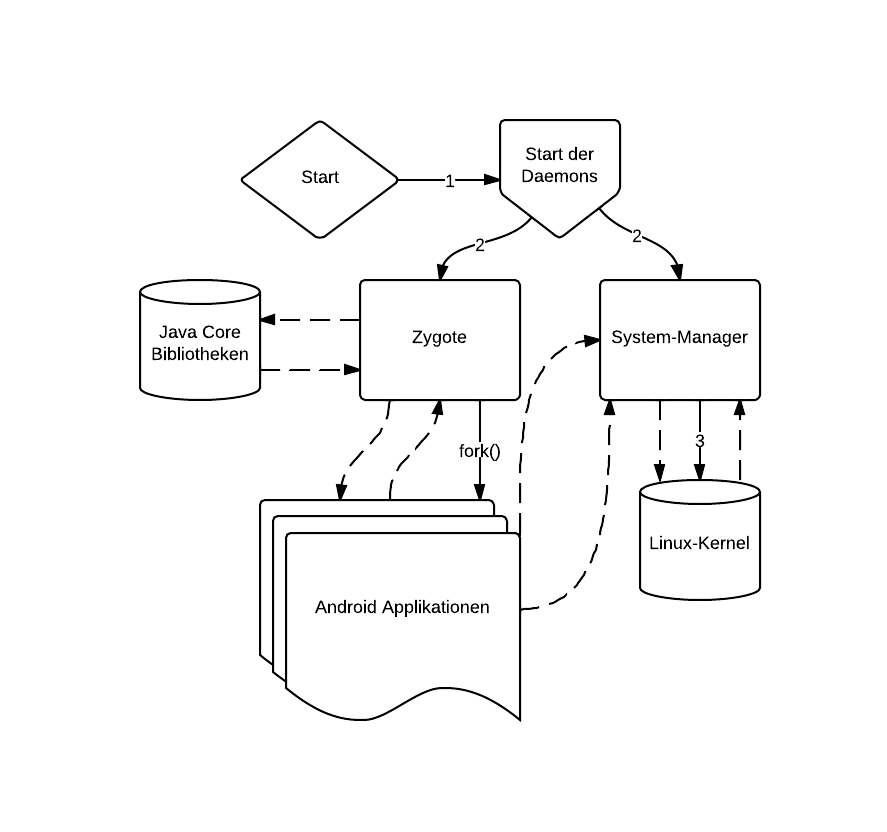
\includegraphics[scale=0.5]{images/dvm}
 \caption{Schematische Darstellung des Starts einer Android Applikation}
 \label{dvm}
 \end{center}
 \end{figure}
 
 Jede Applikation bzw. ihr Prozess verfügt über eine einfache Standard-C-Bibliothek namens \textit{bionic}. Der gesamte Vorgang ist in Abbildung \ref{dvm} dargestellt.
 
 Die gestrichelten Linien beschreiben den Zugriff auf die Hauptkomponenten. Diese sind zum einen die Java Core Bibliotheken und zum anderen der Linux Kernel um bestimmte Hardwarekomponenten zu verwenden.
 
 Eine gewöhnliche VM arbeitet als Stack-Maschine. Diese verfolgt drei Schritte zum Ausführen des Byte-Codes.

 \begin{enumerate}
    \item Der erste Schritt, auch \textit{fetch} genannt, holt ein Befehl vom Stack.
    \item Der nächste Schritt wird als \textit{decode} bezeichnet. In diesem wird abhängig vom Typ des Bytecodes auf Argumente die auf dem Stack liegen zugegriffen.
    \item Der letzte Schritt wird als \textit{execute} bezeichnet. In ihm wird die Funktion des Bytecodes ausgeführt.
 \end{enumerate}
 
 Der Unterschied zwischen der JVM und der DVM liegt in der Art der VM. In der JVM wird die VM durch eine Stack-Maschine realisiert. Die DVM arbeitet als Register-Maschine. Diese holt ihren Bytecode nicht von einem Stack sondern einem - in diesem Fall virtuellen - Register.
 
 Der Vorteil der DVM liegt darin, dass die Registeranzahl und -größe speziell auf ARM-Prozessoren angepasst sind. Des weiteren ist ein Element des Bytecodes der DVM größer als das der JVM.
 
 Jede gestartet Anwendung benötigt Klassen aus der Java-Core-Bibliothek. Der Zygote-Prozess versucht so viele gemeinsam genutzte Klassen in einem geteilten Speicherbereich zu laden um die Speicherbelegung der Applikationen so gering wie möglich zu halten.
 
\subsubsection{Aufbau des Bytecodes}

Der gesamte Bytecode der Android-Applikation sowie der Bytecode der Java-Core-Bibliotheken sind in einen extra für Android entwickelten Format - dem sogenannten \textit{dex} codiert. Dieses unterschiedet sich stark vom \textit{jar}-Format der JVM.

Der Bytecode der DVM ist in Segmente eingeteilt. Die Reihenfolge der einzelnen Segmente ist vorgegeben und muss eingehalten werden. Es gibt insgesamt 9 Segmente die in der Tabelle \ref{segand} erläutert werden.

\begin{table}[h!p]
\begin{tabular}{|p{3cm}|p{11cm}|}\hline

   \textbf{Segmentname} & \textbf{Beschreibung des Segmentes} \\ \hline

   header & Enthält die Versionsnummer und Sicherheitsmerkmale. Alle anderen Segmente sind hier verifiziert und ihre Startadressen vermerkt. \\ \hline

   string\_ids & Zeichenketten die verwendet werden sind hier hinterlegt und haben einen eindeutigen Bezeichner. \\ \hline

   type\_ids & In diesem Segment sind alle Typen (Klassen, Arrays, Elementartypen) definiert unabhängig ob sie verwendet werden oder nicht. \\ \hline

   proto\_ids & Signaturen alle Methoden die in den verschiedenen Klassen verwendet werden. \\ \hline

   fields\_ids & Bezeichner für alle Instanzvariablen unabhängig von ihrer Verwendung. \\ \hline

   methods\_ids & Bezeichner aller Methoden die in der Datei enthalten und verwendet werden. \\ \hline

   class\_ids & Liste aller Klassen und Interfaces.\\ \hline

   data & Datenbereich der alle Informationen der oben genannten Segmenten enthält.\\ \hline
   
   link\_data & Datenbereich für Bindung mit weiteren Dateien. \\ \hline
  
\end{tabular}
\caption{Segmente des Android Bytecodes \cite{eiddvm}}
\label{segand}
\end{table} 
 
 Eine Gegenüberstellung wie in Abbildung \ref{dexjar} macht die wesentlichen Unterschiede im Aufbau des Bytecodes von Java und Android Applikationen ersichtlich.
 
 \begin{figure}[h!t]
 \begin{center}
 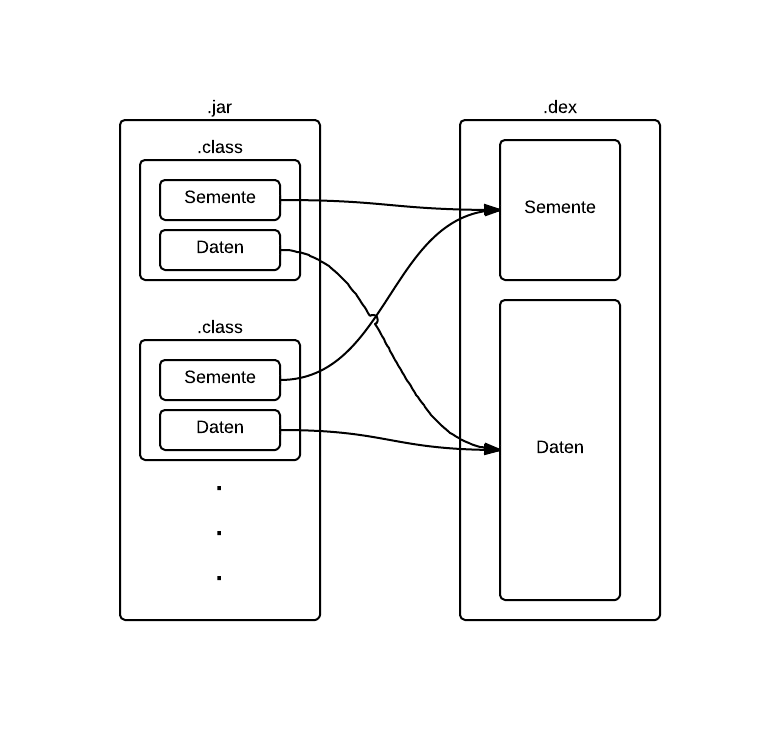
\includegraphics[scale=0.5]{images/dexjar}
 \caption{Gegenüberstellung Java-Bytecode (links) und Android-Bytecode (rechts)}
 \label{dexjar}
 \end{center}
 \end{figure}
 
\subsubsection{Sandbox}
\label{sandbox}

Mit dem Begriff Sandbox\footnote{engl. für Sandkasten} bezeichnet man eine in sich abgeschlossene Umgebung, die prinzipiell keine Auswirkungen auf ihre Umwelt hat. Sandboxes werden häufig als Sicherheitsfeature für Anwendungen oder zum Test von Software verwendet.

Die Anwendung wird dabei vom System, auf dem sie ausgeführt wird abgeschirmt und durch externe Mechanismen kontrolliert. Diese Mechanismen stellen sicher, dass die Anwendung in der Sandbox bleibt und regeln zusätzlich die Informationszufuhr oder den Zugriff auf Systemkomponenten.

Die laufende Anwendung kann diese Mechanismen nicht umgehen oder steuern und ist in ihrem Handlungsspielraum eingeschränkt. Sollte sie jedoch versuchen aus ihrem künstlichen Gefängnis herauszubrechen wird dies durch Sicherungsmaßen erkannt und der Versuch unterbrochen oder die Ausführung der Anwendung gänzlich gestoppt.

\begin{figure}[ht!]
\begin{center}
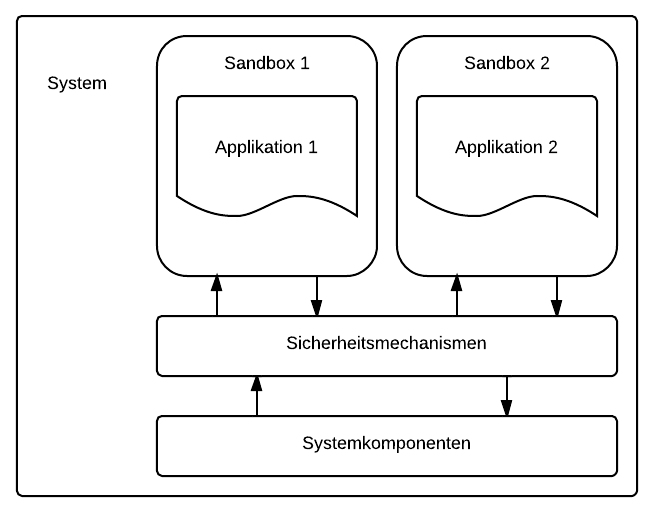
\includegraphics[scale=0.4]{images/sandbox}
\caption{Sandbox-Umgebung mit 2 Applikationen}
\label{sandbox_pic}
\end{center}
\end{figure}

Durch die Verwendung von Sandboxes können nicht nur Softwaretests durchgeführt werden ohne das eigentliche System zu gefährden, sondern auch Anwendungen in Laufzeitumgebungen ausgeführt werden, um die Sicherheit von Daten oder dem eigentlichen System zu gewährleisten. 

Auch Webbrowser verwenden Sandboxes für Webseiten um das System zum Beispiel gegen die Infizierung mit Viren zu schützen. Diese Sandboxes haben auch auf vielen mobilen Endgeräten ihren Platz eingenommen. So werden native Anwendungen auf Mobiltelefonen in Sandboxes ausgeführt um die Anwendungen voneinander abzuschotten und um das System und ihre Komponenten zu schützen. Eine solche Umgebung ist in Abbildung \ref{sandbox_pic} schematisch dargestellt. Sie beschreibt ein System mit mehreren Applikationen und ihren Kommunikationsströmen mit den Systemkomponenten durch mehrere Sandboxes.

\subsubsection{Das Android-Manifest und Permissions}

Die Kommunikation der Sandbox mit der Systemumgebung wird bei Android über \verb+Permissions+ geregelt. Damit werden der Sandbox Benutzungsrechte für genau definierte Bereiche zugeteilt. 
Ein Zentraler Punkt in der Sicherheitsarchitektur von Android besteht darin, dass standardmäßig keine Applikation Berechtigungen besitzt irgendetwas zu tun, was andere Apps, das System oder den Nutzer nachteilig beeinflusst. Darunter fallen beispielsweise der Zugriff auf private Daten des Nutzers oder auf das Netzwerk.

Damit eine Applikation auf das Internet zugreifen kann muss der Entwickler dies aktiv erlauben und der Nutzer bekommt diese Information auch vor dem Installieren angezeigt. Abbildung \ref{permissions} zeigt, wie dem Nutzer bei der Installation die Permissions angezeigt werden, die die Applikation benötigt. 

\begin{figure}[ht!]
\begin{center}
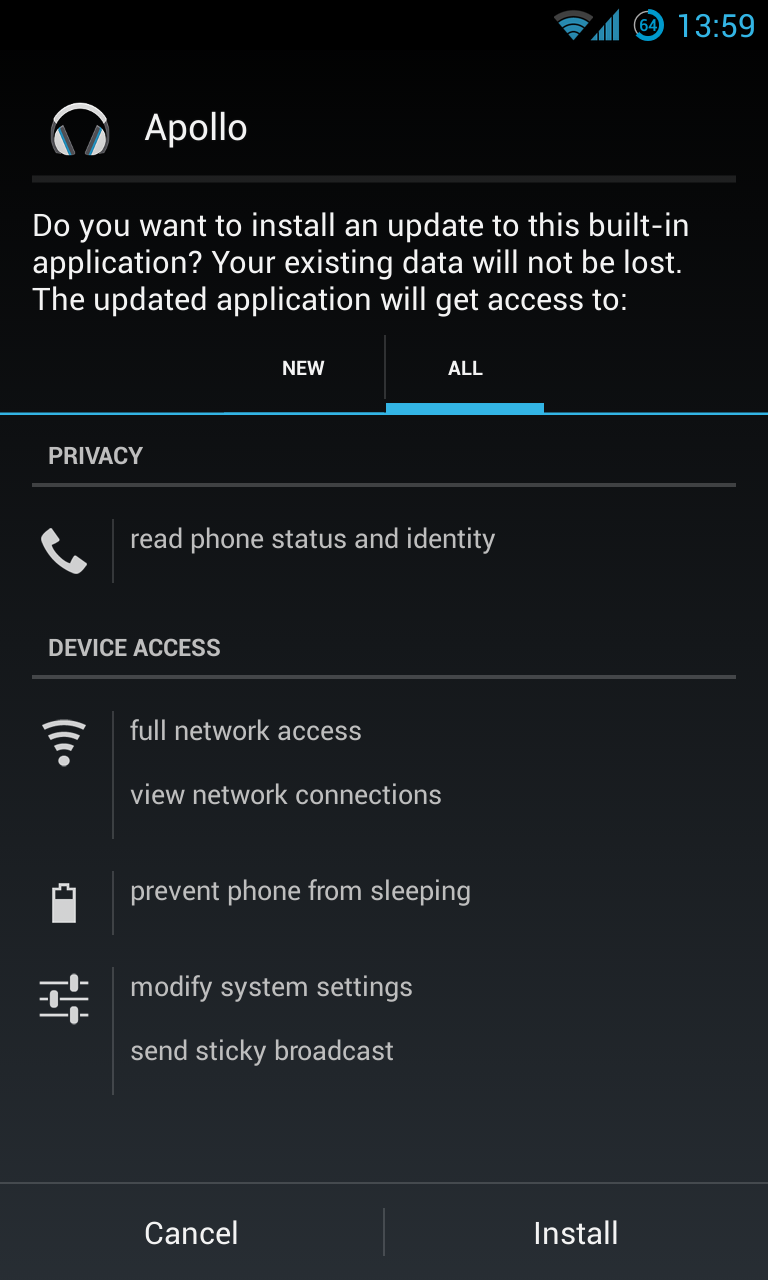
\includegraphics[scale=0.2]{images/permissions}
\caption{Permissions der Applikation Apollo bei der Installation}
\label{permissions}
\end{center}
\end{figure}

Diese Strategie wird konsequent fortgesetzt. So sind automatische Updates nur möglich, wenn sich keine Berechtigungen geändert haben. Falls die App im neusten Update auf die Kontakte zugreifen will muss der Nutzer dies neu bestätigen.

\paragraph{Das Android Manifest}

Jede App hat eine Datei mit dem Namen \verb+AndroidManifest.xml+ in der wichtige Informationen für das System gespeichert werden. Folgende Übersicht zeigt ein paar der wichtigsten Aufgaben des Manifest:

\begin{itemize}
	\item Es beschreibt die Komponenten der Applikation,
	\item Es beinhaltet die verschiedenen Permissions der Applikation,
	\item Es definiert die verwendete Android-Version,
	\item Falls zusätzliche Bibliotheken verwendet werden erscheinen diese auch hier.
\end{itemize}

Somit müssen alle benötigten Permissions in das Manifest eingetragen werden. Bei der Installation kann Android dann diese lesen und dem Nutzer darstellen.

Mit der Transparenz, die dem Nutzer durch diese Strategie gegeben wird, kann zu jedem Zeitpunkt genau entschieden werden, ob eine Applikation sicher ist oder nicht. Entwickler sind durch den \emph{Developer Guide} \cite{android_api} angehalten, die Permissions ihrer Anwendungen so gering wie möglich zu halten. Dadurch werden unnötige Zugriffe und eventuelle Sicherheitslücken vermieden.

\subsection{Komponenten - Die Bestandteile einer Android-Anwendung}
\label{components}

Damit eine Anwendung im Ganzen funktioniert arbeiten mehrere Komponenten zusammen. Alle Arten von Komponenten haben ihre speziellen Aufgaben. In der Folgenden Übersicht werden die beiden Komponentenarten vorgestellt, die in der erstellten Applikation verwendet wurden. (aus \cite{android_components}).

\begin{description}[style=nextline]

	\item[Activities] \hfill \\
	Ein dargestellter Bildschirm mit seinen Elementen wird als \emph{Activity} bezeichnet. Bei der Applikation dieser Arbeit sind beispielsweise die Startseite die angezeigt wird wenn man die das Programm startet oder auch die Player-Ansicht \emph{Activities}.
	
	\item[Services] \hfill \\
	Als \emph{Service} wird eine Komponente bezeichnet, die im Hintergrund läuft und da Aufgaben verrichtet. Der Player der Applikation ist ein Service. Dies bietet die Möglichkeit Musikdateien im Hintergrund zu laden und abzuspielen. So kann der Nutzer beispielsweise im Internet surfen währenddessen das Hörbuch weiter läuft.
	
\end{description}

Zusätzlich zu den Komponenten werden \emph{Ressourcen} zur Verfügung gestellt. Diese beinhalten beispielsweise Bilder und Icons die für die Darstellung verwendet werden.

\subsubsection{Lebenszyklus von Anwendungen}

Jede Komponente hat verschiedene Zustände in denen sie sich befinden kann. Diese Zustände spielen eine große Rolle bei der Entwicklung. 

\begin{figure}[ht!]
\begin{center}
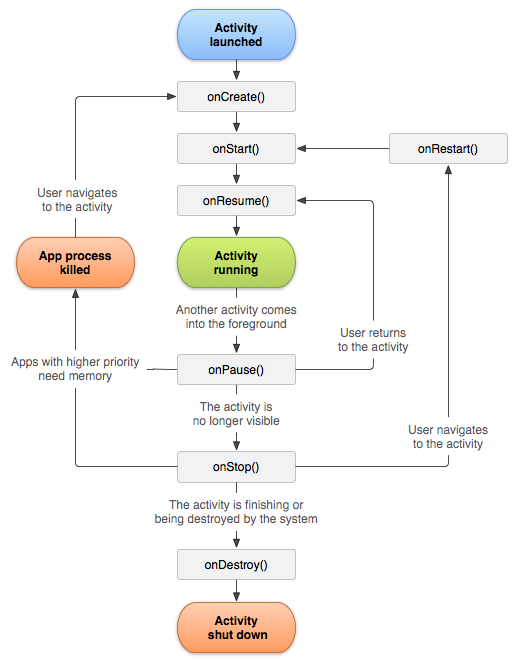
\includegraphics[scale=.6]{images/activity_lifecycle}
\caption{Der Lebenszyklus einer Activity}
\label{lifecycle}
\end{center}
\end{figure}

Grundsätzlich entscheidet man bei Activities in drei Status:

\begin{description}[style=nextline]

	\item[Resumed] \hfill \\
	In diesem Zustand befindet sich die Activity im Vordergrund und ist fokussiert. Wird auch \emph{running} genannt.
	
	\item[Paused] \hfill \\
	Wenn eine andere Activity im Vordergrund ist und die vorherige noch sichtbar ist, ist diese pausiert. Man findet diesen Zustand beispielsweise bei kleinen Auswahlfenstern, bei denen man nach der Auswahl direkt  zur Ausgangs-Activity geleitet wird.
	
	\item[Stopped] \hfill \\
	Die Activity ist im Hintergrund. Der Prozess selbst lebt zwar noch, ist für den Anwender nicht mehr sichtbar und wird nach einer gewissen Zeit vom System komplett beendet.
	
\end{description}

In Abbildung \ref{lifecycle} werden die Status mit den dazugehörigen Übergangsfunktionen angezeigt.

Wichtig bei der Entwicklung ist es, dass man zu jeder Zeit weiß welche Aktion von welchem Zustand aus ausgeführt werden kann. Dabei muss man alle Status beachten und Aktionen dafür festlegen, da es sonst zu ungewolltem Verhalten und Abstürzen kommen kann. Hat man beispielsweise im Status \emph{Activity running} eine Datenbankverbindung geöffnet und vergessen in der \verb+onDestroy()+-Methode diese Verbindung wieder zu schließen, wird die Applikation abstürzen und es kann zu Datenverlust kommen. Dies liegt daran, dass Android die Verbindung nicht selbst beendet. Allerdings stellt es Methoden wie \verb+onDestroy()+ bereit, die aufgerufen wird, wenn die Activity beendet wird, um auf Ereignisse zu reagieren.

Um die Speicherverwaltung muss man sich selbst nicht kümmern. Android verwaltet Speicher selbst. Grundlage dafür bieten die Status der Applikationen. Ist beispielsweise der Browser seit mehreren Minuten im Hintergrund und es wurden zwischenzeitlich mehrere Anwendungen gestartet die Speicher benötigen, wird der Browser beendet um den nötigen RAM zur Verfügung zu stellen. Da aktuelle Geräte über bis zu \SI{3}{GB} Speicher verfügen, kann ein schneller Wechsel zwischen Anwendungen gewährleistet werden, da diese nicht beendet werden müssen.

Allerdings sind Entwickler damit dazu verpflichtet ihre Applikationen dem entsprechend ressourcenschonend und gründlich zu planen, um Abstürze oder eingefrorene Hintergrundanwendungen zu vermeiden.